\documentclass[25pt, a0paper, portrait]{tikzposter}
% \documentclass{tikzposter}
% \geometry{paperwidth=36in,paperheight=44in}
\makeatletter
\setlength{\TP@visibletextwidth}{\textwidth-2\TP@innermargin}
\setlength{\TP@visibletextheight}{\textheight-2\TP@innermargin}
\makeatother


\makeatletter
\newcommand\insertlogoi[2][]{\def\@insertlogoi{\includegraphics[#1]{#2}}}
\newcommand\insertlogoii[2][]{\def\@insertlogoii{\includegraphics[#1]{#2}}}
\newcommand{\tikzpar}{\setlength{\parindent}{5ex}}
\newlength\LogoSep
\setlength\LogoSep{-100pt}

\insertlogoi[width=7cm]{src/D-Pine.eps}
\insertlogoii[width=7cm]{src/Figures/logo_white.png}
% \usetheme{Simple}

\newcounter{tablecounter}
\newenvironment{tikztable}[1][]{
  \def \rememberparameter{#1}
  \vspace{10pt}
  \refstepcounter{tablecounter}
  \begin{center}
  }{
    \ifx\rememberparameter\@empty
    \else
    \\[10pt]
    {\small Tab.~\thetablecounter: \rememberparameter}
    \fi
  \end{center}
}


\renewcommand\maketitle[1][]{  % #1 keys
    \normalsize
    \setkeys{title}{#1}
    % Title dummy to get title height
    \node[transparent,inner sep=\TP@titleinnersep, line width=\TP@titlelinewidth, anchor=north, minimum width=\TP@visibletextwidth-2\TP@titleinnersep]
        (TP@title) at ($(0, 0.5\textheight-\TP@titletotopverticalspace)$) {\parbox{\TP@titlewidth-2\TP@titleinnersep}{\TP@maketitle}};
    \draw let \p1 = ($(TP@title.north)-(TP@title.south)$) in node {
        \setlength{\TP@titleheight}{\y1}
        \setlength{\titleheight}{\y1}
        \global\TP@titleheight=\TP@titleheight
        \global\titleheight=\titleheight
    };

    % Compute title position
    \setlength{\titleposleft}{-0.5\titlewidth}
    \setlength{\titleposright}{\titleposleft+\titlewidth}
    \setlength{\titlepostop}{0.5\textheight-\TP@titletotopverticalspace}
    \setlength{\titleposbottom}{\titlepostop-\titleheight}

    % Title style (background)
    \TP@titlestyle

    % Title node
    \node[inner sep=\TP@titleinnersep, line width=\TP@titlelinewidth, anchor=north, minimum width=\TP@visibletextwidth-2\TP@titleinnersep]
        at (0,0.5\textheight-\TP@titletotopverticalspace)
        (title)
        {\parbox{\TP@titlewidth-2\TP@titleinnersep}{\TP@maketitle}};

    \node[inner sep=0pt,anchor=west] 
      at ([xshift=-\LogoSep]title.west)
      {\@insertlogoi};

    \node[inner sep=0pt,anchor=east] 
      at ([xshift=\LogoSep]title.east)
      {\@insertlogoii};

    % Settings for blocks
    \normalsize
    \setlength{\TP@blocktop}{\titleposbottom-\TP@titletoblockverticalspace}
}
\makeatother

\definecolorstyle{sampleColorStyle} {
	\definecolor{colorOne}{named}{white}
	\definecolor{colorTwo}{named}{red}
	\definecolor{colorThree}{named}{red}
	\definecolor{Dgreen}{HTML}{00693e}
}{
	% Background Colors
	\colorlet{backgroundcolor}{colorOne}
	\colorlet{framecolor}{white}
	% Title Colors
	\colorlet{titlefgcolor}{white}
	\colorlet{titlebgcolor}{Dgreen}
	% Block Colors
	\colorlet{blocktitlebgcolor}{white}
	\colorlet{blocktitlefgcolor}{Dgreen}
	\colorlet{blockbodybgcolor}{white}
	\colorlet{blockbodyfgcolor}{black}
	% Innerblock Colors
	\colorlet{innerblocktitlebgcolor}{white}
	\colorlet{innerblocktitlefgcolor}{black}
	\colorlet{innerblockbodybgcolor}{colorThree!30!white}
	\colorlet{innerblockbodyfgcolor}{black}
	% Note colors
	\colorlet{notefgcolor}{black}
	\colorlet{notebgcolor}{colorTwo!50!white}
	\colorlet{noteframecolor}{colorTwo}
}

\definelayouttheme{sample}{
	\usecolorstyle[colorPalette=sampleColorPalette]{sampleColorStyle}
	\usebackgroundstyle{sample}
	\usetitlestyle{Test}
	\useblockstyle{Simple}
	\useinnerblockstyle{Simple}
	\usenotestyle{Corner}
}

\usetheme{sample}

% \begin{document}
%\geometry{paperwidth=44in,paperheight=36in}
\usetitlestyle{Filled}
\title{
\begin{minipage}{\textwidth}
   \centering
   Chemically Self-Consistent Isochrones
   \\
   \bigskip
   \mbox{of the Globular Cluster NGC 2808}
 \end{minipage}
 }
% \title{Updated High-Temperature Opacities for The Dartmouth Stellar Evolution Program and their Effect on the Jao Gap Location}
\author{Emily M. Boudreaux$^{1}$, Renata Edeas Hoh$^{1}$, Brian C. Chaboyer$^{1}$, \& Gregory Feiden$^{2}$}
\institute{{$^{1}$Department of Physics and Astronomy, Dartmouth College, Hanover, NH 03755, USA}\\{$^{2}$Department of Physics and Astronomy, University of North Georgia, Dahlonega, GA 30533, USA}}
\usepackage[utf8]{inputenc}
\usepackage{wrapfig}
\usepackage{amsmath}
\usepackage{setspace}
\usepackage{fontspec}
\usepackage[T1]{fontenc}
\usepackage{adjustbox}
\usepackage{tikz}
\usepackage{xcolor}

\tikzposterlatexaffectionproofoff

\begin{document}
	\maketitle
	\begin{columns}
	  \column{0.33}

		\block{Abstract}{\fontsize{38}{45}\selectfont
      \tikzpar The inferred helium mass fraction of multiple populations (MPs) in
      globular clusters (GCs) can vary significantly from older to younger
      populations {\color{blue}[1]}. As the origin of these MPs remains an open question, and one
      which is sensitive to the compositional variations between populations,
      the extent of the composition variations is a key parameter when
      constraining formation channels. Many metal abundances may be directly
      measured spectroscopically; however, helium abundances are not directly
      observable in GCs. Instead, helium abundances are inferred from stellar
      models. It is therefore important to build stellar models which are
      chemically self-consistent between the structure, atmosphere, and
      opacities. In this work we present the first chemically self-consistent
      stellar models of the Milky Way globular cluster NGC 2808. We find that
      the helium abundance of the second generation of stars is enhanced when
      compared to the first generation by 9 percent.
    }

    \block{Consistency \& Modeling}{\fontsize{38}{45}\selectfont
	    \vspace{-5mm}
      
      \tikzpar We use the Dartmouth stellar evolution program (DSEP) {\color{blue}[2]} to evolve
      a grid of models with a variety of mixing lengths and helium mass
      fractions. Atmospheric boundary conditions are computed using MARCS {\color{blue}[3]} 
      and are kept chemically consistent with the structure code from hydrogen
      to zinc. High-Temperature opacities are pulled from OPLIB and low
      temperature opacities are pulled from Aesopus, both of these are also
      kept chemically consistent from hydrogen to zinc.

	    }
    \block{\texttt{FIDANKA}}{\fontsize{38}{45}\selectfont
	    \vspace{-5mm}
      
      The software we develop for this work (\texttt{fidanka}) has been
      released under a permissive open-source licence and is available on
      GitHub.

      \begin{tikzfigure}[Concept map of \texttt{fidanka}]
        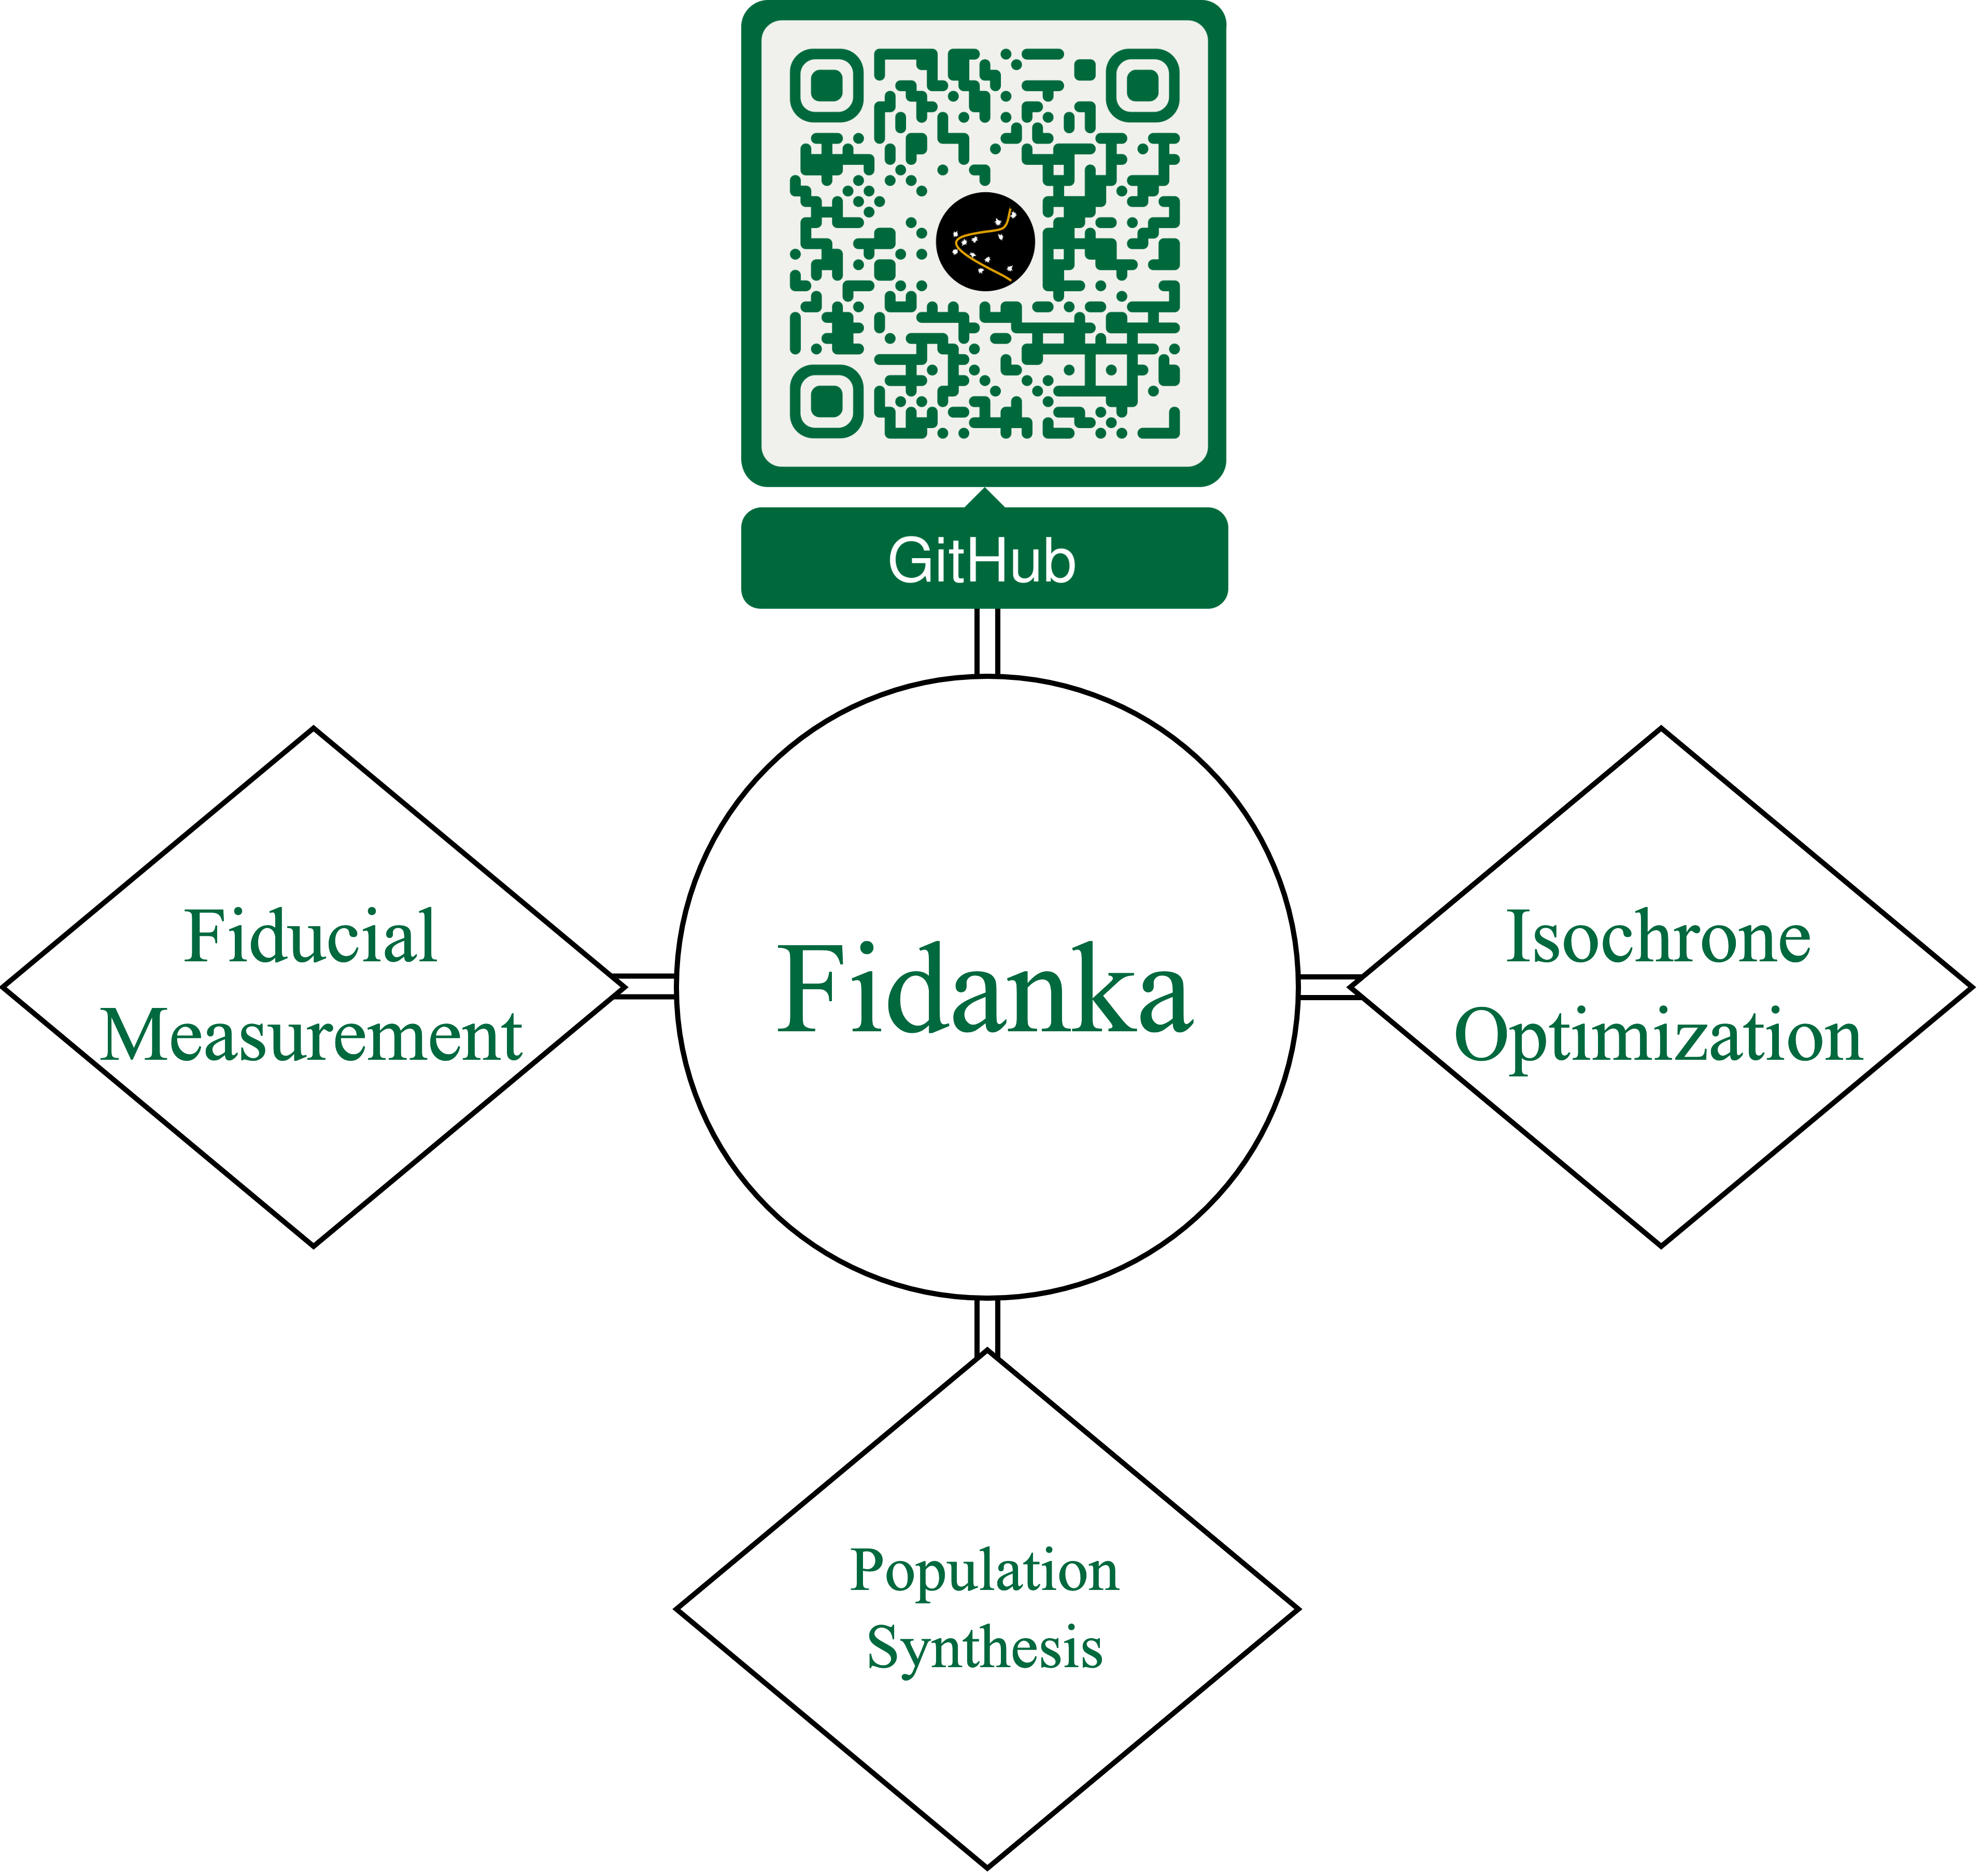
\includegraphics[width=0.28\textwidth]{src/Figures/FidankaSale.png}
      \end{tikzfigure}


	    }

	  \column{0.66}
    \block{Fiducial Measurement}{\fontsize{38}{45}\selectfont
      \tikzpar In order to measure the subtle number density variations separating
      populations along the Main Sequence we make use of a novel, convex-hull
      based, adaptive binning approach. This algorithm keeps the number of stars
      per bin uniform. An example of the density estimate produced by this
      algorithm is shown in Figure 2. \textbf{Note how the sequences stand out clearly
      in the density plot.}

      \begin{tikzfigure}[NGC 2808 CMD from the HUGS survey after data quality cuts have been applied (top). Number density of stars in the CMD of NGC 2808 (bottom).]
        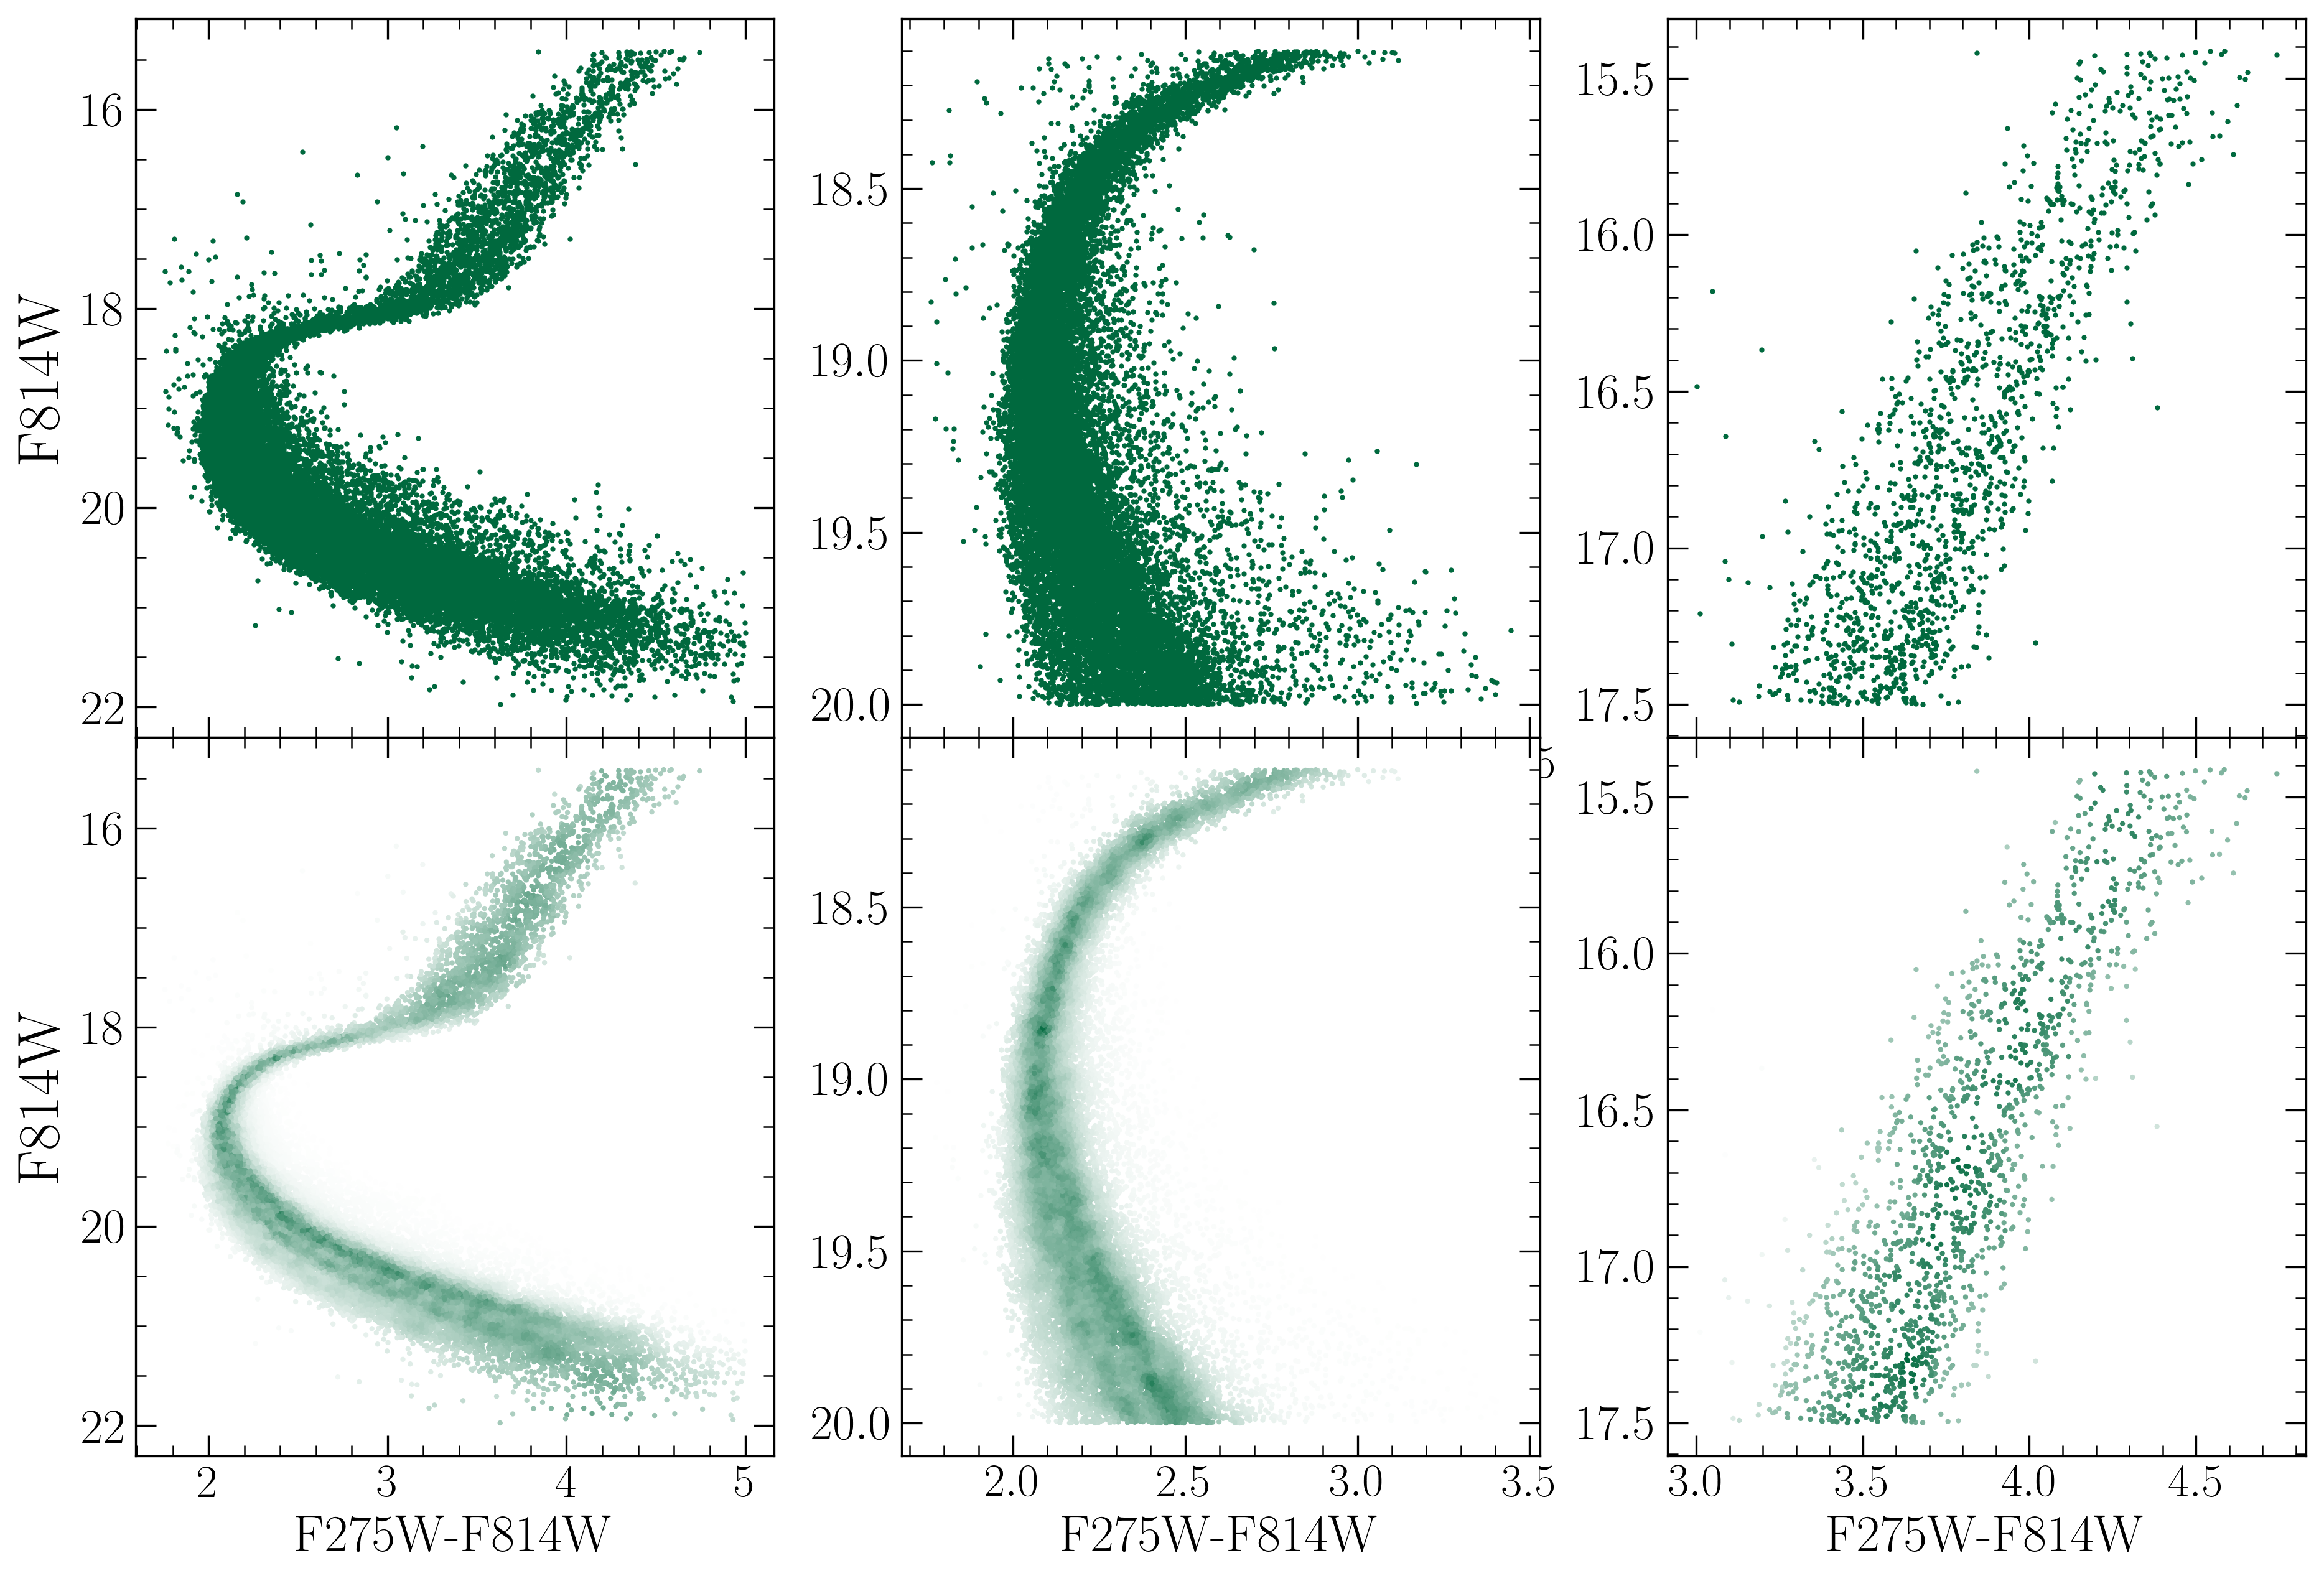
\includegraphics[width=0.6\textwidth]{src/Figures/NBFigs/DensityMap.png}
      \end{tikzfigure}

			\begin{minipage}[t]{0.40\linewidth}
      \tikzpar We use Bayesian Gaussian Mixture Modeling
      and the Diecrelt Process to trace median ridge lines over a series of
      magnitude bins. This eliminates the need for a prior on the exact number of
      populations. Traced fiducial lines for the two most extreme populations
        (A\&E in {\color{blue}[4]}) in NGC 2808 are shown in in Figure 3.
			\end{minipage}%
			\begin{adjustbox}{valign=t}
        \begin{minipage}[t]{0.66\linewidth}
          \begin{tikzfigure}[NGC 2808 populations A \& E median ridge lines measured using fidanka.]
            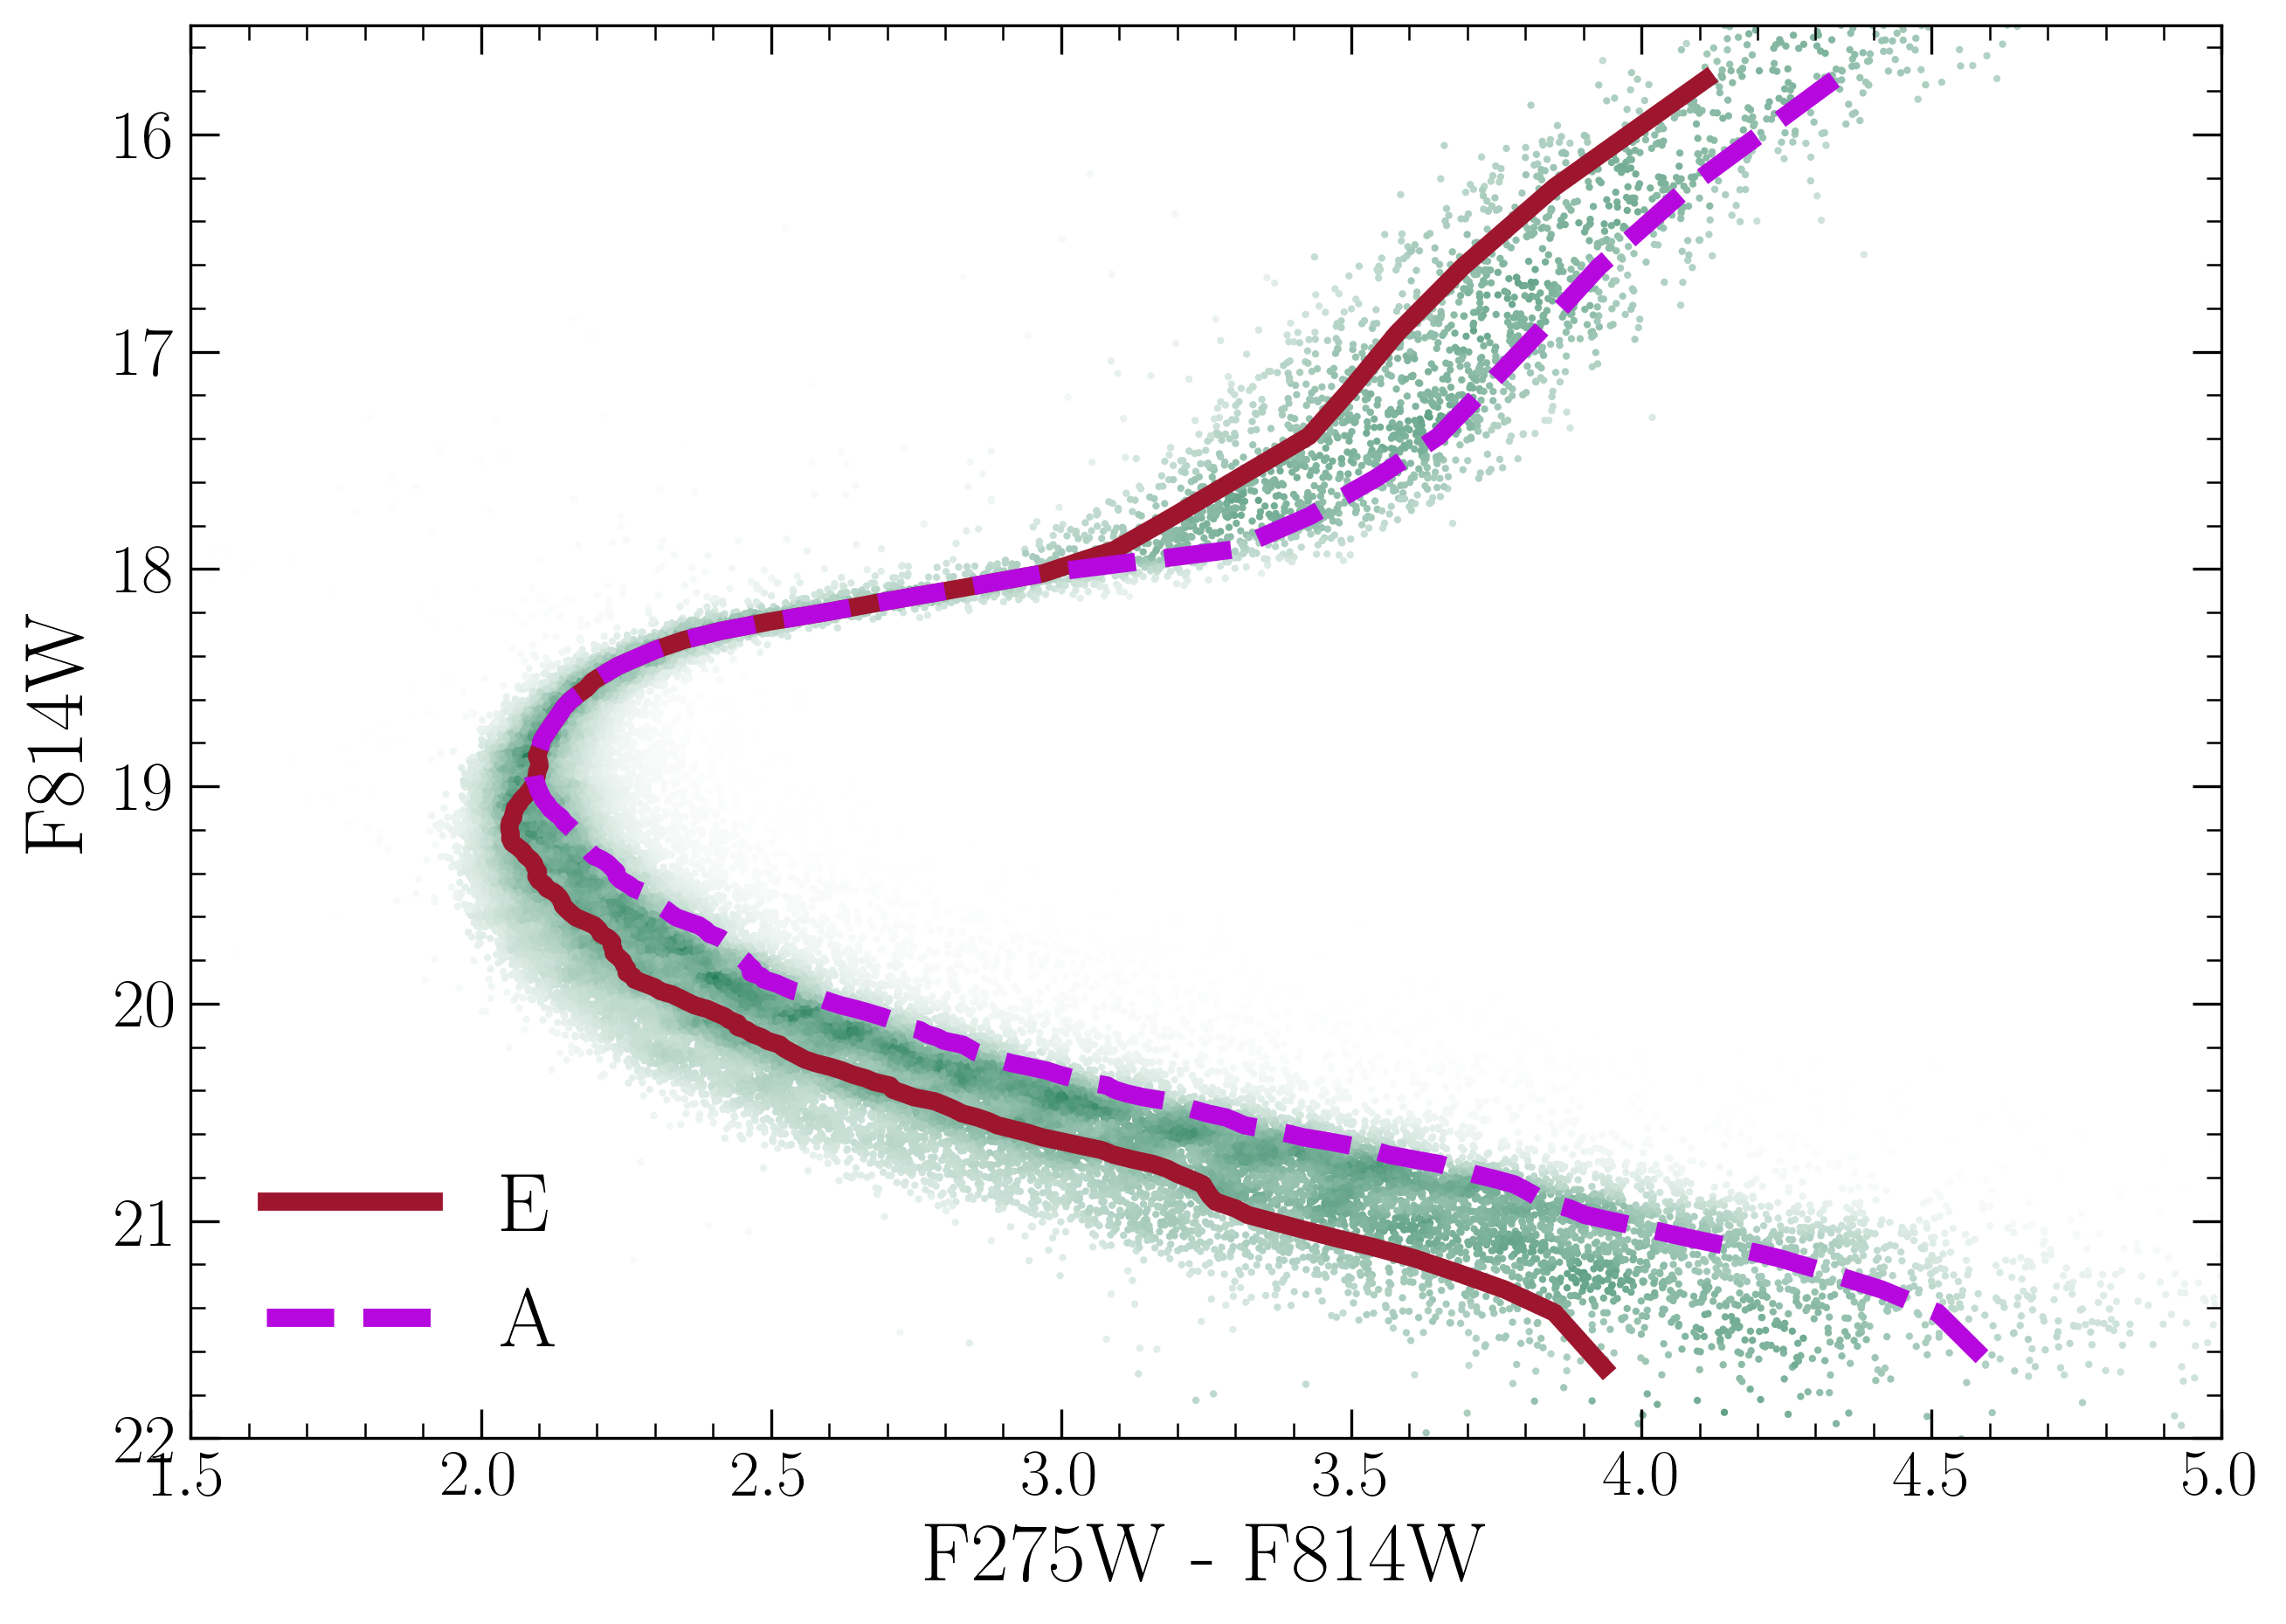
\includegraphics[scale=1]{src/Figures/NBFigs/NGC2808Fid.png}
          \end{tikzfigure}
        \end{minipage}
			\end{adjustbox}

      \vspace{5mm}

			\begin{adjustbox}{valign=t}

        \hspace{-3cm}

        \begin{minipage}[t]{0.60\linewidth}
          \begin{tikzfigure}[Preliminary best fitting isochrones. The discontinuity near color=2.9 is due to discrepencies between FreeEOS and an ideal EOS. Work is ongoing to resolve this prior to publication.]
            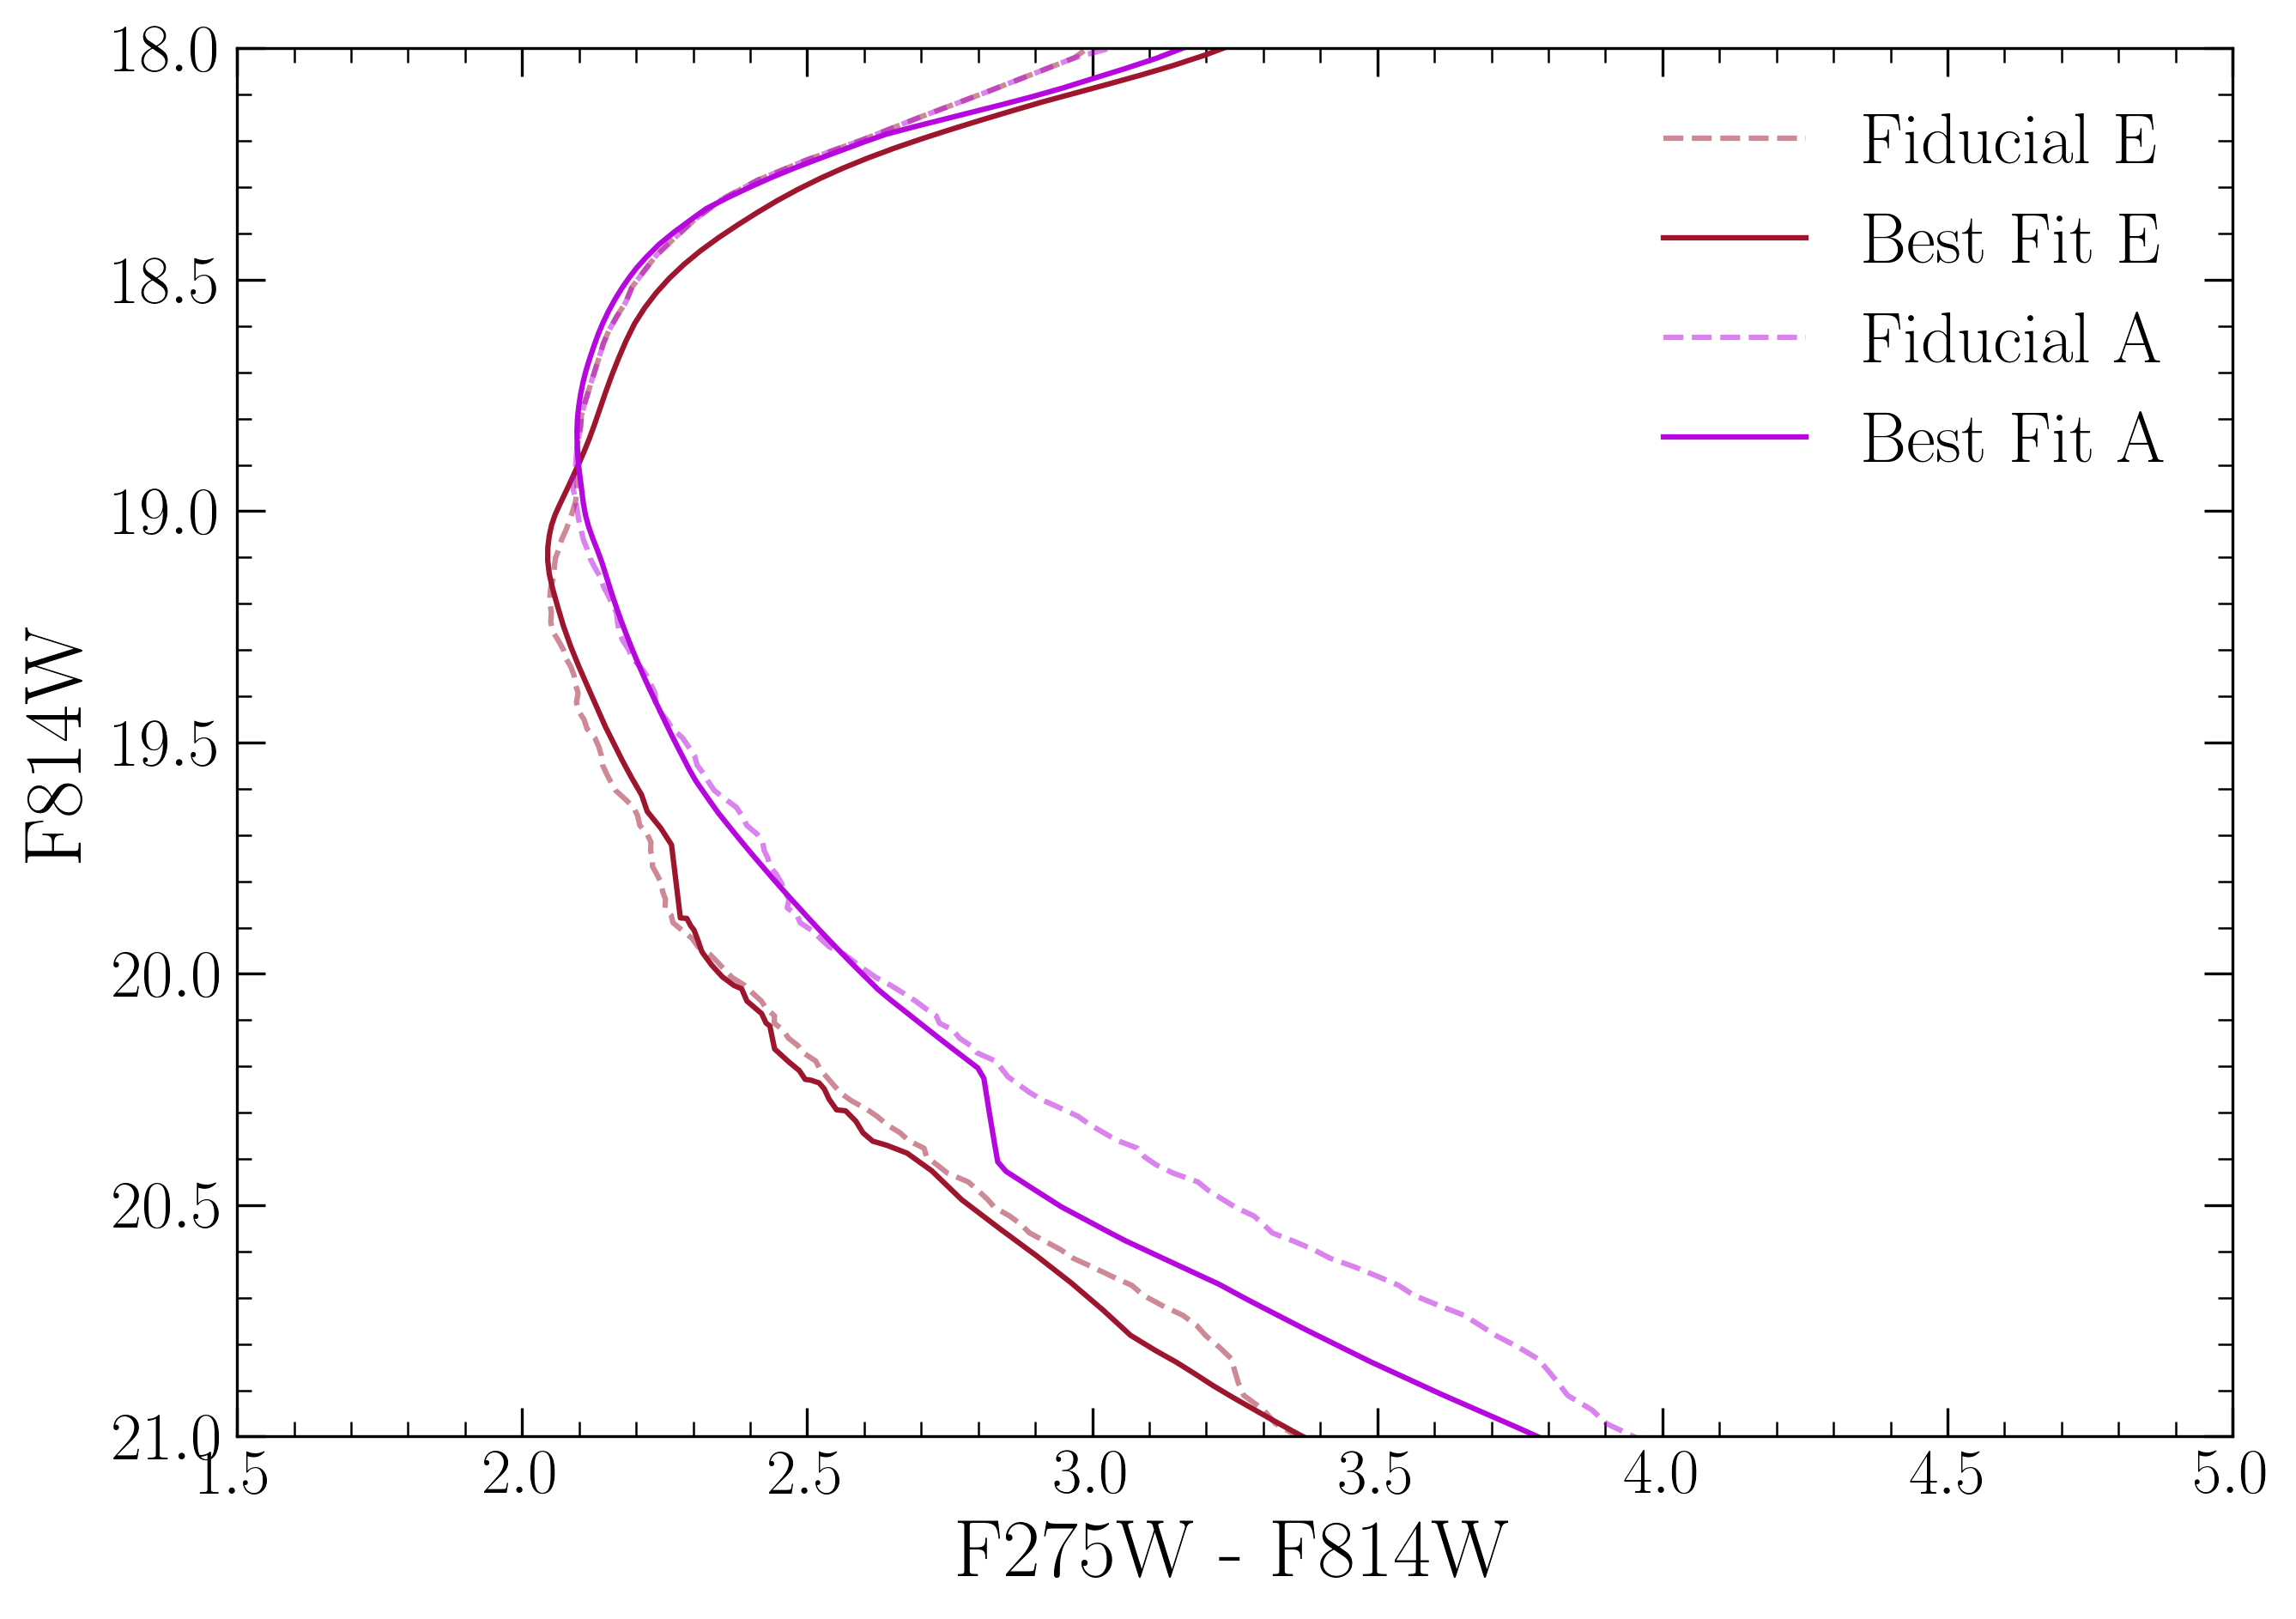
\includegraphics[scale=1]{src/Figures/NBFigs/BestFit.png}
          \end{tikzfigure}
        \end{minipage}
			\end{adjustbox}
			\begin{minipage}[t]{0.45\linewidth}
        Using the path from the fast dynamic time warping algorithm {\color{blue}[5]} as an
        objective function we fit the optimal distance modulus, B-V color
        excess, and age for NGC 2808. Best fitting isochrones are shown in
        Figure 4. We find $\mu = 15.01$, $E(B-V)=0.43$, and age=11.81 Gyr ($\chi^{2}_{\nu} = 0.067)$. \textbf{We
        find preliminary best fit helium mass fractions of Y=0.36 for Population E and
        Y=0.27 for population A. These are consistent with past results from
        the literature.}
			\end{minipage}%
    }

    \block{}{%

    \vspace{-2.5cm}

      \begin{center}
        \begin{minipage}{0.45\linewidth}
          We acknowledge the support of a NASA grant (No. 80NSSC18K0634) and
          JWST GO Grant (No. GO-02560). Additionally, we would like to thank
          James Colgan, Elisabeth Newton, and Aaron Dotter for their assistance
          with this work. Finally, we would like to thank Aylin Garcia Soto,
          Keighley Rockcliffe, Rayna Rampalli, Stephanie Podjed, and Kara
          Fagerstrom for their useful discussion related to this work. 
        \end{minipage}\hfill
        \begin{minipage}{0.45\linewidth}
          {\fontsize{24}{22}\selectfont
          \begin{enumerate}
            \item Piotto, G., Bedin, L. R., Anderson, J., et al. 2007, \textit{ApJ} Letters, 661, L53
            \item Dotter, A., Chaboyer, B., Jevremovi ́c, D., et al. 2008, \textit{ApJ} Supplement Series, 178, 89 
            \item Gustafsson B., Edvardsson B., Eriksson K., Jørgensen U.G., Nordlund Å., Plez B. 2008, \textit{A\&A} 486, 951
            \item Milone, A. P., Marino, A. F., Piotto, G., et al. 2015, \textit{ApJ}, 808, 51
            \item Stan Salvador, and Philip Chan. 2007, \textit{Intelligent Data Analysis}, 561-580.
          \end{enumerate}
          }
        \end{minipage}
      \end{center}
    }
	\end{columns}
\end{document}
